\chapter{Vectorization}
 \label{chap:vec}
 
 To mitigate the duplicated storage of data in both PyNEST and the NestKernel that was explained at the end of \autoref{chap:jit}, we have decomposed the models into segments that are simple to generate from the perspective of the code generator and yet independent, which makes them more efficient in the JIT code generation context. In computer science, we refer to such a decomposition as \emph{modularity}. The idea behind it is to consider the model as an aggregation of blocks, and these blocks are assembled during the progress of the simulation script upon calling the \texttt{Create()}, \texttt{Connect()} and \texttt{Simulate()} functions.
 
 \begin{figure}[ht!]
 \centering 
\tikzset{every picture/.style={line width=0.75pt}} %set default line width to 0.75pt        

\tikzset{every picture/.style={line width=0.75pt}} %set default line width to 0.75pt        
\scalebox{0.5}{
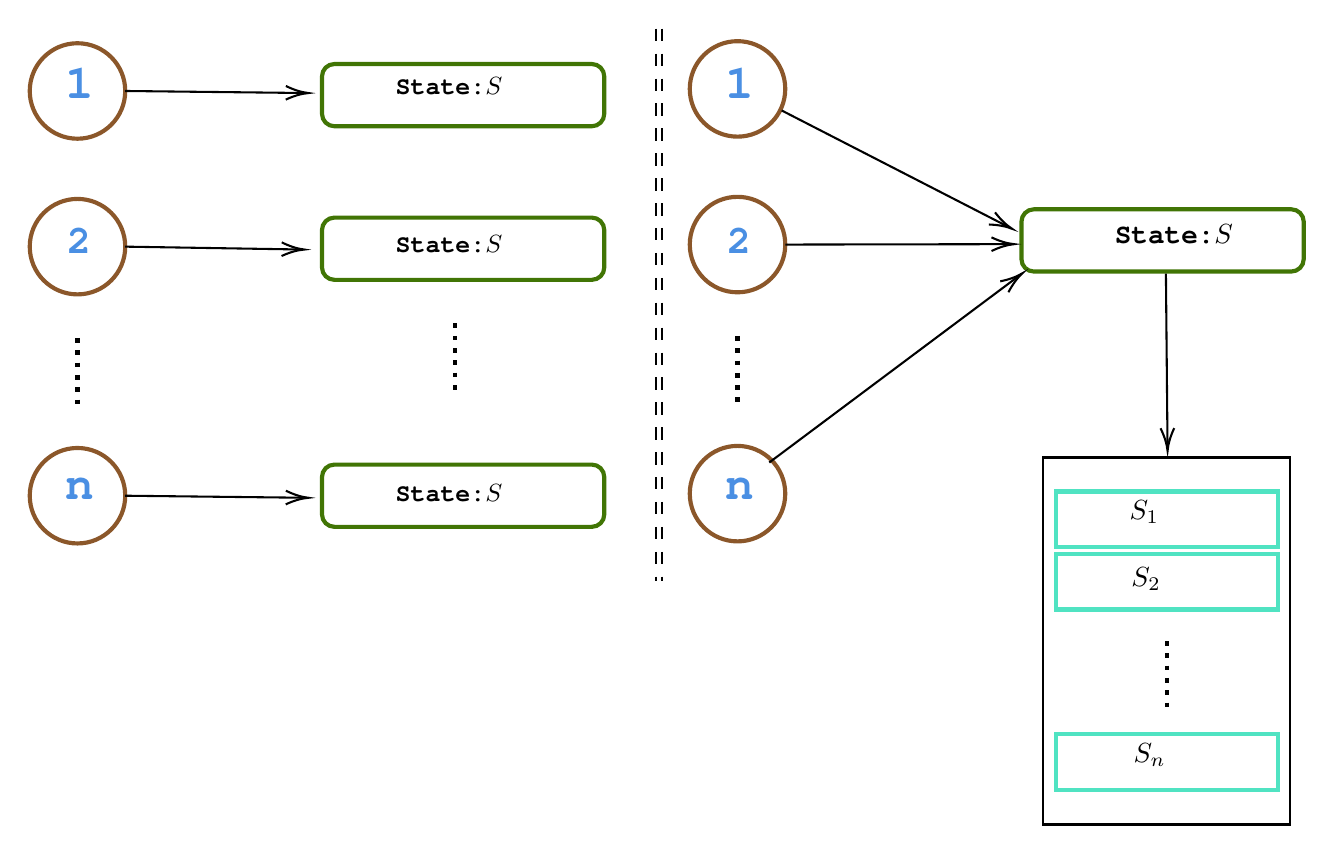
\begin{tikzpicture}[x=0.75pt,y=0.75pt,yscale=-1,xscale=1]
%uncomment if require: \path (0,407); %set diagram left start at 0, and has height of 407

%Straight Lines [id:da55454641213535] 
\draw  [dash pattern={on 4.5pt off 4.5pt}]  (320.3,5) -- (320.3,271)(317.3,5) -- (317.3,271) ;
%Shape: Circle [id:dp8702862076063935] 
\draw  [color={rgb, 255:red, 139; green, 87; blue, 42 }  ,draw opacity=1 ][line width=1.5]  (15.5,35) .. controls (15.5,22.3) and (25.8,12) .. (38.5,12) .. controls (51.2,12) and (61.5,22.3) .. (61.5,35) .. controls (61.5,47.7) and (51.2,58) .. (38.5,58) .. controls (25.8,58) and (15.5,47.7) .. (15.5,35) -- cycle ;
%Shape: Circle [id:dp7392015554996889] 
\draw  [color={rgb, 255:red, 139; green, 87; blue, 42 }  ,draw opacity=1 ][line width=1.5]  (15.5,110) .. controls (15.5,97.3) and (25.8,87) .. (38.5,87) .. controls (51.2,87) and (61.5,97.3) .. (61.5,110) .. controls (61.5,122.7) and (51.2,133) .. (38.5,133) .. controls (25.8,133) and (15.5,122.7) .. (15.5,110) -- cycle ;
%Shape: Circle [id:dp2317183663755913] 
\draw  [color={rgb, 255:red, 139; green, 87; blue, 42 }  ,draw opacity=1 ][line width=1.5]  (15.5,230) .. controls (15.5,217.3) and (25.8,207) .. (38.5,207) .. controls (51.2,207) and (61.5,217.3) .. (61.5,230) .. controls (61.5,242.7) and (51.2,253) .. (38.5,253) .. controls (25.8,253) and (15.5,242.7) .. (15.5,230) -- cycle ;
%Straight Lines [id:da38894787507587125] 
\draw [line width=1.5]  [dash pattern={on 1.69pt off 2.76pt}]  (38.5,154) -- (38.5,189) ;
%Shape: Circle [id:dp12642715215459321] 
\draw  [color={rgb, 255:red, 139; green, 87; blue, 42 }  ,draw opacity=1 ][line width=1.5]  (333.5,34) .. controls (333.5,21.3) and (343.8,11) .. (356.5,11) .. controls (369.2,11) and (379.5,21.3) .. (379.5,34) .. controls (379.5,46.7) and (369.2,57) .. (356.5,57) .. controls (343.8,57) and (333.5,46.7) .. (333.5,34) -- cycle ;
%Shape: Circle [id:dp810070044573385] 
\draw  [color={rgb, 255:red, 139; green, 87; blue, 42 }  ,draw opacity=1 ][line width=1.5]  (333.5,109) .. controls (333.5,96.3) and (343.8,86) .. (356.5,86) .. controls (369.2,86) and (379.5,96.3) .. (379.5,109) .. controls (379.5,121.7) and (369.2,132) .. (356.5,132) .. controls (343.8,132) and (333.5,121.7) .. (333.5,109) -- cycle ;
%Shape: Circle [id:dp9280679238307532] 
\draw  [color={rgb, 255:red, 139; green, 87; blue, 42 }  ,draw opacity=1 ][line width=1.5]  (333.5,229) .. controls (333.5,216.3) and (343.8,206) .. (356.5,206) .. controls (369.2,206) and (379.5,216.3) .. (379.5,229) .. controls (379.5,241.7) and (369.2,252) .. (356.5,252) .. controls (343.8,252) and (333.5,241.7) .. (333.5,229) -- cycle ;
%Straight Lines [id:da15371263291441517] 
\draw [line width=1.5]  [dash pattern={on 1.69pt off 2.76pt}]  (356.5,153) -- (356.5,188) ;
%Rounded Rect [id:dp7336088599348931] 
\draw  [color={rgb, 255:red, 65; green, 117; blue, 5 }  ,draw opacity=1 ][line width=1.5]  (156.3,28) .. controls (156.3,24.69) and (158.99,22) .. (162.3,22) -- (286.3,22) .. controls (289.61,22) and (292.3,24.69) .. (292.3,28) -- (292.3,46) .. controls (292.3,49.31) and (289.61,52) .. (286.3,52) -- (162.3,52) .. controls (158.99,52) and (156.3,49.31) .. (156.3,46) -- cycle ;
%Rounded Rect [id:dp7973935185576317] 
\draw  [color={rgb, 255:red, 65; green, 117; blue, 5 }  ,draw opacity=1 ][line width=1.5]  (156.3,102) .. controls (156.3,98.69) and (158.99,96) .. (162.3,96) -- (286.3,96) .. controls (289.61,96) and (292.3,98.69) .. (292.3,102) -- (292.3,120) .. controls (292.3,123.31) and (289.61,126) .. (286.3,126) -- (162.3,126) .. controls (158.99,126) and (156.3,123.31) .. (156.3,120) -- cycle ;
%Rounded Rect [id:dp24096719551443324] 
\draw  [color={rgb, 255:red, 65; green, 117; blue, 5 }  ,draw opacity=1 ][line width=1.5]  (156.3,221) .. controls (156.3,217.69) and (158.99,215) .. (162.3,215) -- (286.3,215) .. controls (289.61,215) and (292.3,217.69) .. (292.3,221) -- (292.3,239) .. controls (292.3,242.31) and (289.61,245) .. (286.3,245) -- (162.3,245) .. controls (158.99,245) and (156.3,242.31) .. (156.3,239) -- cycle ;
%Straight Lines [id:da10099325819440153] 
\draw [line width=1.5]  [dash pattern={on 1.69pt off 2.76pt}]  (220.3,147) -- (220.3,182) ;
%Straight Lines [id:da41136869587104075] 
\draw    (61.5,35) -- (147.8,35.98) ;
\draw [shift={(149.8,36)}, rotate = 180.65] [color={rgb, 255:red, 0; green, 0; blue, 0 }  ][line width=0.75]    (10.93,-3.29) .. controls (6.95,-1.4) and (3.31,-0.3) .. (0,0) .. controls (3.31,0.3) and (6.95,1.4) .. (10.93,3.29)   ;
%Straight Lines [id:da2870462219518801] 
\draw    (61.5,110) -- (145.8,111.37) ;
\draw [shift={(147.8,111.4)}, rotate = 180.93] [color={rgb, 255:red, 0; green, 0; blue, 0 }  ][line width=0.75]    (10.93,-3.29) .. controls (6.95,-1.4) and (3.31,-0.3) .. (0,0) .. controls (3.31,0.3) and (6.95,1.4) .. (10.93,3.29)   ;
%Straight Lines [id:da05926760400293096] 
\draw    (61.5,230) -- (147.8,230.98) ;
\draw [shift={(149.8,231)}, rotate = 180.65] [color={rgb, 255:red, 0; green, 0; blue, 0 }  ][line width=0.75]    (10.93,-3.29) .. controls (6.95,-1.4) and (3.31,-0.3) .. (0,0) .. controls (3.31,0.3) and (6.95,1.4) .. (10.93,3.29)   ;
%Rounded Rect [id:dp5327938345694794] 
\draw  [color={rgb, 255:red, 65; green, 117; blue, 5 }  ,draw opacity=1 ][line width=1.5]  (493.3,98) .. controls (493.3,94.69) and (495.99,92) .. (499.3,92) -- (623.3,92) .. controls (626.61,92) and (629.3,94.69) .. (629.3,98) -- (629.3,116) .. controls (629.3,119.31) and (626.61,122) .. (623.3,122) -- (499.3,122) .. controls (495.99,122) and (493.3,119.31) .. (493.3,116) -- cycle ;
%Straight Lines [id:da24962287312365405] 
\draw    (377.8,44.4) -- (487.02,100.49) ;
\draw [shift={(488.8,101.4)}, rotate = 207.18] [color={rgb, 255:red, 0; green, 0; blue, 0 }  ][line width=0.75]    (10.93,-3.29) .. controls (6.95,-1.4) and (3.31,-0.3) .. (0,0) .. controls (3.31,0.3) and (6.95,1.4) .. (10.93,3.29)   ;
%Straight Lines [id:da0756642394053797] 
\draw    (379.5,109) -- (487.8,108.8) ;
\draw [shift={(489.8,108.8)}, rotate = 179.9] [color={rgb, 255:red, 0; green, 0; blue, 0 }  ][line width=0.75]    (10.93,-3.29) .. controls (6.95,-1.4) and (3.31,-0.3) .. (0,0) .. controls (3.31,0.3) and (6.95,1.4) .. (10.93,3.29)   ;
%Straight Lines [id:da5803854131041157] 
\draw    (371.8,214) -- (492.2,124) ;
\draw [shift={(493.8,122.8)}, rotate = 143.22] [color={rgb, 255:red, 0; green, 0; blue, 0 }  ][line width=0.75]    (10.93,-3.29) .. controls (6.95,-1.4) and (3.31,-0.3) .. (0,0) .. controls (3.31,0.3) and (6.95,1.4) .. (10.93,3.29)   ;
%Shape: Rectangle [id:dp8303325304778635] 
\draw  [color={rgb, 255:red, 80; green, 227; blue, 194 }  ,draw opacity=1 ][line width=1.5]  (509.9,228) -- (616.7,228) -- (616.7,254.8) -- (509.9,254.8) -- cycle ;
%Straight Lines [id:da8940404822400119] 
\draw [line width=1.5]  [dash pattern={on 1.69pt off 2.76pt}]  (563.3,300) -- (563.3,335) ;
%Shape: Rectangle [id:dp9884603058041568] 
\draw  [color={rgb, 255:red, 80; green, 227; blue, 194 }  ,draw opacity=1 ][line width=1.5]  (509.9,258) -- (616.7,258) -- (616.7,284.8) -- (509.9,284.8) -- cycle ;
%Shape: Rectangle [id:dp5121717716613057] 
\draw  [color={rgb, 255:red, 80; green, 227; blue, 194 }  ,draw opacity=1 ][line width=1.5]  (509.9,345) -- (616.7,345) -- (616.7,371.8) -- (509.9,371.8) -- cycle ;
%Shape: Rectangle [id:dp907132490388713] 
\draw   (503.8,211.6) -- (622.8,211.6) -- (622.8,388.4) -- (503.8,388.4) -- cycle ;
%Straight Lines [id:da8778275970204104] 
\draw    (562.9,123) -- (563.68,206.4) ;
\draw [shift={(563.7,208.4)}, rotate = 269.46] [color={rgb, 255:red, 0; green, 0; blue, 0 }  ][line width=0.75]    (10.93,-3.29) .. controls (6.95,-1.4) and (3.31,-0.3) .. (0,0) .. controls (3.31,0.3) and (6.95,1.4) .. (10.93,3.29)   ;

% Text Node
\draw (31,23) node [anchor=north west][inner sep=0.75pt]   [align=left] {{\fontfamily{pcr}\selectfont {\LARGE \textcolor[rgb]{0.29,0.56,0.89}{\textbf{1}}}}};
% Text Node
\draw (32,100) node [anchor=north west][inner sep=0.75pt]   [align=left] {{\fontfamily{pcr}\selectfont {\Large \textcolor[rgb]{0.29,0.56,0.89}{\textbf{2}}}}};
% Text Node
\draw (31,220) node [anchor=north west][inner sep=0.75pt]   [align=left] {{\fontfamily{pcr}\selectfont {\LARGE \textcolor[rgb]{0.29,0.56,0.89}{\textbf{n}}}}};
% Text Node
\draw (349,23) node [anchor=north west][inner sep=0.75pt]   [align=left] {{\fontfamily{pcr}\selectfont {\LARGE \textcolor[rgb]{0.29,0.56,0.89}{\textbf{1}}}}};
% Text Node
\draw (350,100) node [anchor=north west][inner sep=0.75pt]   [align=left] {{\fontfamily{pcr}\selectfont {\Large \textcolor[rgb]{0.29,0.56,0.89}{\textbf{2}}}}};
% Text Node
\draw (349,220) node [anchor=north west][inner sep=0.75pt]   [align=left] {{\fontfamily{pcr}\selectfont {\LARGE \textcolor[rgb]{0.29,0.56,0.89}{\textbf{n}}}}};
% Text Node
\draw (536.8,98) node [anchor=north west][inner sep=0.75pt]   [align=left] {{\fontfamily{pcr}\selectfont \textbf{State:$S$}}};
% Text Node
\draw (190.3,27) node [anchor=north west][inner sep=0.75pt]   [align=left] {{\small {\fontfamily{pcr}\selectfont \textbf{State:$S$}}}};
% Text Node
\draw (190.3,103) node [anchor=north west][inner sep=0.75pt]   [align=left] {{\small {\fontfamily{pcr}\selectfont \textbf{State:$S$ }}}};
% Text Node
\draw (190.3,223) node [anchor=north west][inner sep=0.75pt]   [align=left] {{\small {\fontfamily{pcr}\selectfont \textbf{State:$S$ }}}};
% Text Node
\draw (544.8,263) node [anchor=north west][inner sep=0.75pt]   [align=left] {$S_2$};
% Text Node
\draw (543.9,231) node [anchor=north west][inner sep=0.75pt]   [align=left] {$S_{1}$};
% Text Node
\draw (545.9,348) node [anchor=north west][inner sep=0.75pt]   [align=left] {$S_{n}$};
\end{tikzpicture}
}
\caption{\textbf{Modularity and Vectorization}: The left part represents the current implementation of the models in the NestKernel. We have $n$ instances of the model and each has its own state block with an attribute $S$. In the right, we have the suggested idea using vectorization. All instances share the same state block, and instead of having $n$ separate attributes, the attributes are aggregated in a single array with size $n$.}
\label{fig:moduliarity_vectorization}
\end{figure}

Each model instance will start as a \emph{dummy} instance of the \texttt{Node} class in the NestKernel that has pointers to the blocks, which will be assigned separately and independently during the simulation. Such blocks may extend the dummy instance by new attributes like new Parameters and new \emph{States}, or even new functions related to updating the state of the model, delivering emitted events and registering connections. One valid partitioning of the model into segments would be the partition that aligns with the \texttt{Create()}, \texttt{Connect()} and \texttt{Simulate()} functions. When calling the \texttt{Create()} function, we would only require the \emph{parameter} and \emph{state blocks} to be assigned to the model. Upon \texttt{Connect()}, we would extend the model by new functions that support the connectivity of the neuron with the synapse. Finally, by calling \texttt{Simulate()}, we would append the \emph{update block}. This partition might not be always perfect and depending on the chosen model, we may require a different segmentation and a more detailed analysis to create the blocks. 

One problem that might arise with this approach is the time it takes to assign all the blocks to all the instances upon creation, connection setup and prior to the simulation. Imagine we are creating $n$ instances of a specific model. Using the modularity concept as depicted in the left panel of \autoref{fig:moduliarity_vectorization}, this  means that each state block must be constructed separately, and each block must be assigned to each instance of the model. Assuming the time for creating a State block is $c$, binding each instance of the model with the block takes time $a$ and $l$ would be the time needed for creating each node separately, then the overall time we will spend is $n \cdot (c + a + l)$ for connecting each block with its corresponding instance.

A solution to this problem presents itself in the form of \emph{vectorization}. Instead of having $n$ instances of the state block, we could only use a single block that is \emph{shared} among all instances of the model. If the state block is vectorized (i.e., consists of a vector of attributes), each entry in the vector belongs to one instance of the model at the position $i$. For the example above, if we again have $n$ instances, the overall time needed for creating the instances is $ \mathcal{O}(n \cdot (a + l) + c + r )$, where $r$ is the overhead for resizing the vector and allocating space for it when new instances are added. By only having a single central entity that has direct access to the blocks and instances of the model, it is possible to reduce the $n \cdot a$ component drastically and arrive at an overall time of $ \mathcal{O}(n \cdot l + c + r) $ for calls to \texttt{Create()}.

\begin{figure}[ht!]
    \centering
    
\tikzset{every picture/.style={line width=0.75pt}} %set default line width to 0.75pt        
\scalebox{0.5}{
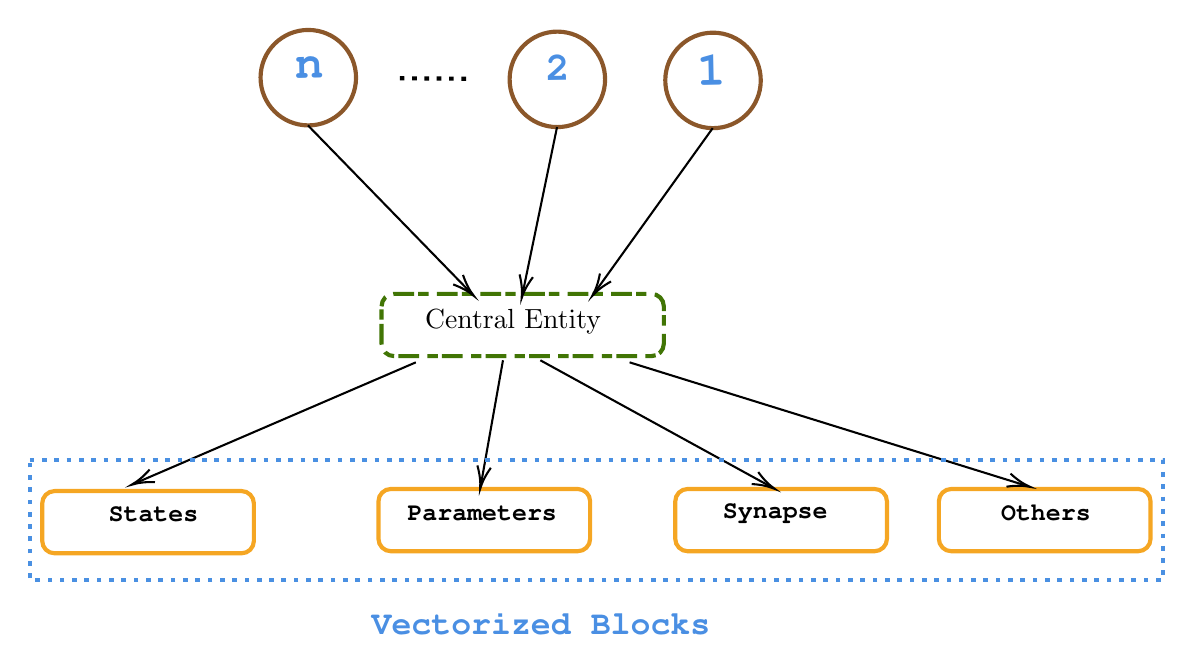
\begin{tikzpicture}[x=0.75pt,y=0.75pt,yscale=-1,xscale=1]
%uncomment if require: \path (0,498); %set diagram left start at 0, and has height of 498

%Shape: Circle [id:dp8800281867294899] 
\draw  [color={rgb, 255:red, 139; green, 87; blue, 42 }  ,draw opacity=1 ][line width=1.5]  (422.15,8.16) .. controls (434.86,8.25) and (445.08,18.62) .. (445,31.32) .. controls (444.91,44.02) and (434.54,54.25) .. (421.84,54.16) .. controls (409.14,54.08) and (398.91,43.71) .. (399,31.01) .. controls (399.08,18.3) and (409.45,8.08) .. (422.15,8.16) -- cycle ;
%Shape: Circle [id:dp5741608202490043] 
\draw  [color={rgb, 255:red, 139; green, 87; blue, 42 }  ,draw opacity=1 ][line width=1.5]  (347.16,7.65) .. controls (359.86,7.74) and (370.09,18.11) .. (370,30.81) .. controls (369.91,43.51) and (359.55,53.74) .. (346.84,53.65) .. controls (334.14,53.57) and (323.91,43.2) .. (324,30.5) .. controls (324.09,17.79) and (334.45,7.57) .. (347.16,7.65) -- cycle ;
%Shape: Circle [id:dp5967106723538562] 
\draw  [color={rgb, 255:red, 139; green, 87; blue, 42 }  ,draw opacity=1 ][line width=1.5]  (227.16,6.84) .. controls (239.86,6.92) and (250.09,17.29) .. (250,29.99) .. controls (249.92,42.7) and (239.55,52.92) .. (226.85,52.84) .. controls (214.14,52.75) and (203.92,42.38) .. (204,29.68) .. controls (204.09,16.98) and (214.46,6.75) .. (227.16,6.84) -- cycle ;
%Straight Lines [id:da29612448901916677] 
\draw [line width=1.5]  [dash pattern={on 1.69pt off 2.76pt}]  (303,30.35) -- (268,30.12) ;
%Rounded Rect [id:dp817325473851275] 
\draw  [color={rgb, 255:red, 65; green, 117; blue, 5 }  ,draw opacity=1 ][dash pattern={on 3.75pt off 3pt on 7.5pt off 1.5pt}][line width=1.5]  (262.3,140) .. controls (262.3,136.69) and (264.99,134) .. (268.3,134) -- (392.3,134) .. controls (395.61,134) and (398.3,136.69) .. (398.3,140) -- (398.3,158) .. controls (398.3,161.31) and (395.61,164) .. (392.3,164) -- (268.3,164) .. controls (264.99,164) and (262.3,161.31) .. (262.3,158) -- cycle ;
%Straight Lines [id:da2876052096679098] 
\draw    (226.85,52.84) -- (305.41,133.57) ;
\draw [shift={(306.8,135)}, rotate = 225.78] [color={rgb, 255:red, 0; green, 0; blue, 0 }  ][line width=0.75]    (10.93,-3.29) .. controls (6.95,-1.4) and (3.31,-0.3) .. (0,0) .. controls (3.31,0.3) and (6.95,1.4) .. (10.93,3.29)   ;
%Straight Lines [id:da21493226208984018] 
\draw    (346.84,53.65) -- (330.21,134.04) ;
\draw [shift={(329.8,136)}, rotate = 281.69] [color={rgb, 255:red, 0; green, 0; blue, 0 }  ][line width=0.75]    (10.93,-3.29) .. controls (6.95,-1.4) and (3.31,-0.3) .. (0,0) .. controls (3.31,0.3) and (6.95,1.4) .. (10.93,3.29)   ;
%Straight Lines [id:da8022220076746627] 
\draw    (421.84,54.16) -- (364.97,133.38) ;
\draw [shift={(363.8,135)}, rotate = 305.68] [color={rgb, 255:red, 0; green, 0; blue, 0 }  ][line width=0.75]    (10.93,-3.29) .. controls (6.95,-1.4) and (3.31,-0.3) .. (0,0) .. controls (3.31,0.3) and (6.95,1.4) .. (10.93,3.29)   ;
%Rounded Rect [id:dp8286030826901589] 
\draw  [color={rgb, 255:red, 245; green, 166; blue, 35 }  ,draw opacity=1 ][line width=1.5]  (98.8,235) .. controls (98.8,231.69) and (101.49,229) .. (104.8,229) -- (194.8,229) .. controls (198.11,229) and (200.8,231.69) .. (200.8,235) -- (200.8,253) .. controls (200.8,256.31) and (198.11,259) .. (194.8,259) -- (104.8,259) .. controls (101.49,259) and (98.8,256.31) .. (98.8,253) -- cycle ;
%Rounded Rect [id:dp8880914545431386] 
\draw  [color={rgb, 255:red, 245; green, 166; blue, 35 }  ,draw opacity=1 ][line width=1.5]  (260.8,234) .. controls (260.8,230.69) and (263.49,228) .. (266.8,228) -- (356.8,228) .. controls (360.11,228) and (362.8,230.69) .. (362.8,234) -- (362.8,252) .. controls (362.8,255.31) and (360.11,258) .. (356.8,258) -- (266.8,258) .. controls (263.49,258) and (260.8,255.31) .. (260.8,252) -- cycle ;
%Rounded Rect [id:dp6892742079278225] 
\draw  [color={rgb, 255:red, 245; green, 166; blue, 35 }  ,draw opacity=1 ][line width=1.5]  (403.8,234) .. controls (403.8,230.69) and (406.49,228) .. (409.8,228) -- (499.8,228) .. controls (503.11,228) and (505.8,230.69) .. (505.8,234) -- (505.8,252) .. controls (505.8,255.31) and (503.11,258) .. (499.8,258) -- (409.8,258) .. controls (406.49,258) and (403.8,255.31) .. (403.8,252) -- cycle ;
%Rounded Rect [id:dp7219152508117417] 
\draw  [color={rgb, 255:red, 245; green, 166; blue, 35 }  ,draw opacity=1 ][line width=1.5]  (530.8,234) .. controls (530.8,230.69) and (533.49,228) .. (536.8,228) -- (626.8,228) .. controls (630.11,228) and (632.8,230.69) .. (632.8,234) -- (632.8,252) .. controls (632.8,255.31) and (630.11,258) .. (626.8,258) -- (536.8,258) .. controls (533.49,258) and (530.8,255.31) .. (530.8,252) -- cycle ;
%Straight Lines [id:da25677235530600573] 
\draw    (278.8,167) -- (143.64,225.21) ;
\draw [shift={(141.8,226)}, rotate = 336.7] [color={rgb, 255:red, 0; green, 0; blue, 0 }  ][line width=0.75]    (10.93,-3.29) .. controls (6.95,-1.4) and (3.31,-0.3) .. (0,0) .. controls (3.31,0.3) and (6.95,1.4) .. (10.93,3.29)   ;
%Straight Lines [id:da5461915180486876] 
\draw    (320.8,166) -- (310.15,226.03) ;
\draw [shift={(309.8,228)}, rotate = 280.06] [color={rgb, 255:red, 0; green, 0; blue, 0 }  ][line width=0.75]    (10.93,-3.29) .. controls (6.95,-1.4) and (3.31,-0.3) .. (0,0) .. controls (3.31,0.3) and (6.95,1.4) .. (10.93,3.29)   ;
%Straight Lines [id:da447748925987298] 
\draw    (338.8,166) -- (450.05,227.04) ;
\draw [shift={(451.8,228)}, rotate = 208.75] [color={rgb, 255:red, 0; green, 0; blue, 0 }  ][line width=0.75]    (10.93,-3.29) .. controls (6.95,-1.4) and (3.31,-0.3) .. (0,0) .. controls (3.31,0.3) and (6.95,1.4) .. (10.93,3.29)   ;
%Straight Lines [id:da09082598278343812] 
\draw    (381.8,167) -- (572.89,226.41) ;
\draw [shift={(574.8,227)}, rotate = 197.27] [color={rgb, 255:red, 0; green, 0; blue, 0 }  ][line width=0.75]    (10.93,-3.29) .. controls (6.95,-1.4) and (3.31,-0.3) .. (0,0) .. controls (3.31,0.3) and (6.95,1.4) .. (10.93,3.29)   ;
%Shape: Rectangle [id:dp8214226950203147] 
\draw  [color={rgb, 255:red, 74; green, 144; blue, 226 }  ,draw opacity=1 ][dash pattern={on 1.69pt off 2.76pt}][line width=1.5]  (92.8,214) -- (638.8,214) -- (638.8,272) -- (92.8,272) -- cycle ;

% Text Node
\draw (412.67,18.30) node [anchor=north west][inner sep=0.75pt]  [rotate=-358.84] [align=left] {{\fontfamily{pcr}\selectfont {\LARGE \textcolor[rgb]{0.29,0.56,0.89}{\textbf{1}}}}};
% Text Node
\draw (339.79,18.27) node [anchor=north west][inner sep=0.75pt]  [rotate=-359.07] [align=left] {{\fontfamily{pcr}\selectfont {\Large \textcolor[rgb]{0.29,0.56,0.89}{\textbf{2}}}}};
% Text Node
\draw (219.13,18.30) node [anchor=north west][inner sep=0.75pt]  [rotate=-358.67] [align=left] {{\fontfamily{pcr}\selectfont {\LARGE \textcolor[rgb]{0.29,0.56,0.89}{\textbf{n}}}}};
% Text Node
\draw (281.8,140) node [anchor=north west][inner sep=0.75pt]   [align=left] {Central Entity};
% Text Node
\draw (129.3,235) node [anchor=north west][inner sep=0.75pt]   [align=left] {{\fontfamily{pcr}\selectfont \textbf{{\small States}}}};
% Text Node
\draw (273.3,235) node [anchor=north west][inner sep=0.75pt]   [align=left] {{\fontfamily{pcr}\selectfont {\small \textbf{Parameters}}}};
% Text Node
\draw (425.3,234) node [anchor=north west][inner sep=0.75pt]   [align=left] {{\small \textbf{{\fontfamily{pcr}\selectfont Synapse}}}};
% Text Node
\draw (559.3,234) node [anchor=north west][inner sep=0.75pt]   [align=left] {{\fontfamily{pcr}\selectfont {\small \textbf{Others}}}};
% Text Node
\draw (256,286) node [anchor=north west][inner sep=0.75pt]   [align=left] {{\fontfamily{pcr}\selectfont {\large \textbf{\textcolor[rgb]{0.29,0.56,0.89}{Vectorized Blocks}}}}};

\end{tikzpicture}
}
    \caption{\textbf{Modularity with a central entity}: The model is segmented into different blocks that are assembled together during the simulating. The nodes share the central entity that manages the state of the blocks. Each of the blocks supports vectorization, and each of the attributes has a vector form with a size equal to the created population in the network from the specified model.}
    \label{fig:central_entity}
\end{figure}

In \autoref{fig:central_entity}, we illustrate the best way how the modularity and vectorization may work together to achieve a simple and flexible data structure for handling models in the NestKernel. The central entity in this context may be the \texttt{Model} class in the \texttt{NestKernel}, which anyway only exists once per thread. The instances of the \texttt{Node} class are depicted as circles that all share the central entity, which has direct access to the state and parameter blocks. Each node has a local ID with which it can retrieve information about the currently stored values at the corresponding position in the vector.
 
In this thesis, we will only focus on implementing the vectorization concept for the models of the neurons and show that it is possible to integrate the vectorization design in the NestKernel without drastically modifying the overall workflow. The extension to the synapses and further data structures is left for a follow-up project.

In this chapter, we first introduce a naïve solution and discuss its drawbacks and then show how the drawbacks can be addressed in a way that respects the requirements coming from the NestKernel and finally discuss the current limitations and how is it possible to mitigate them.

\section{The Data Structure}

Vectorization in a plain language is the process of rewriting an instruction that is repeating $n$ times over single entities to an instruction that is processing $k$ entities simultaneously. Usually, the term vectorization overlaps with the term \emph{SIMD}, which is the short form of \emph{single instruction/multiple data}, and refers to the capability of the hardware components to perform the same operation on multiple data fields concurrently. \autoref{fig:simd} illustrates a simple example of SIMD executing four operations in parallel. Another term strongly related to high performance computing and optimization is the term \emph{speedup}. The term speedup in the context of vectorization is the ratio between the time required by the \emph{non-vectorized} operation $T(1)$ and the time required by the vectorized operation, executing $k$ operations at the same time (denoted $T(k)$). The speedup is defined as $$S(k) = \frac{T(1)}{T(k)}$$. Assuming that a single instance of the operation takes $t$ units to complete and also neglecting the overhead of memory access, then applying the operation on $n$ elements we have $T(1) = n \cdot t$ and $T(k) = \frac{n}{k} \cdot t$, which implies $$S(k) = \frac{T(1)}{T(k)} = \frac{n \cdot t}{\frac{n}{k} \cdot t} = k.$$

A speedup of $k$ means that we load $k$ elements into the register of the processor and execute the operation $k$ times in parallel. In reality, the larger $k$ gets, the less speedup we can expect, as we have a limited memory bandwidth, limited number of registers and a limited number of parallel processing units.

\begin{figure}[ht!]
\centering
\tikzset{every picture/.style={line width=0.75pt}} %set default line width to 0.75pt        
\scalebox{0.5}{
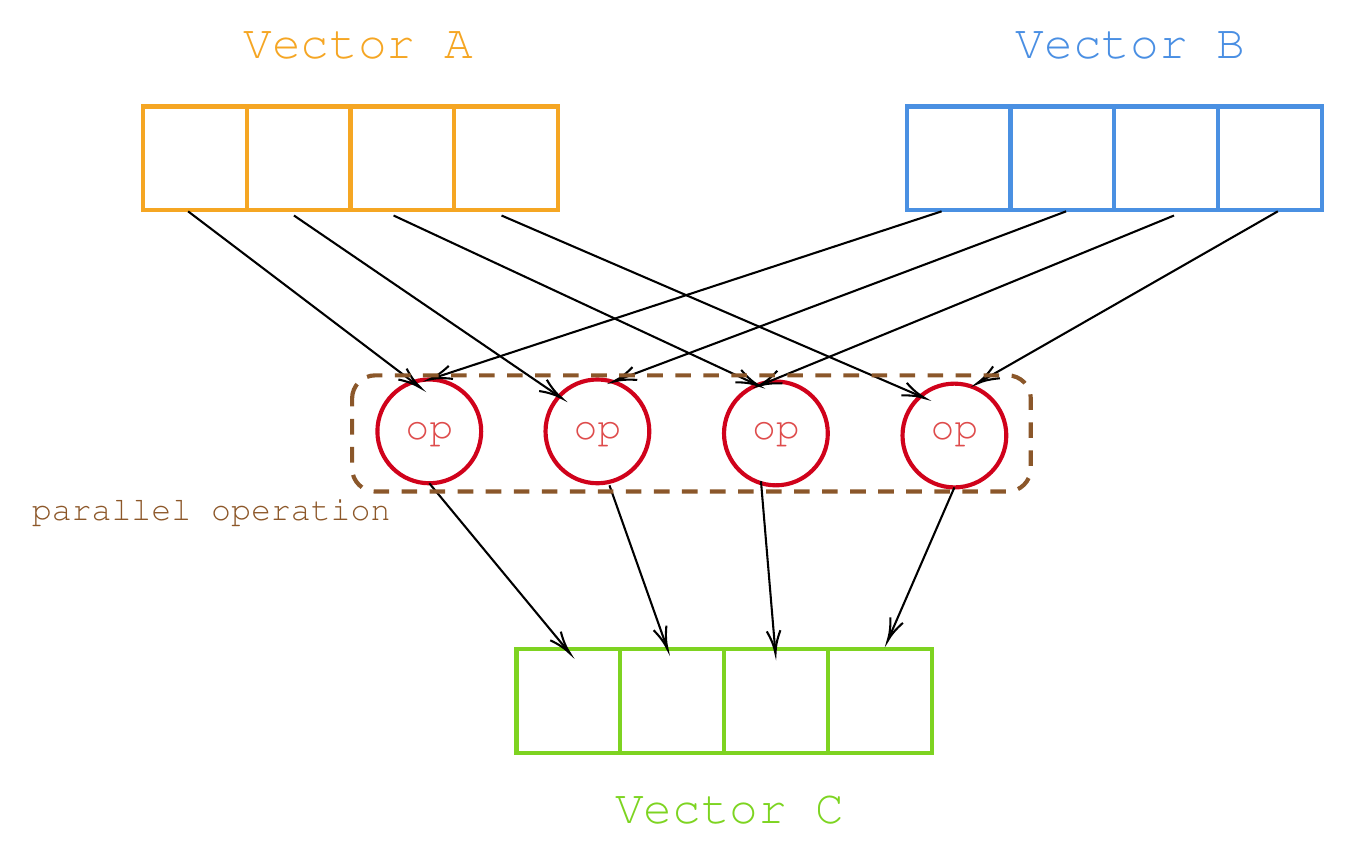
\begin{tikzpicture}[x=0.75pt,y=0.75pt,yscale=-1,xscale=1]
%uncomment if require: \path (0,489); %set diagram left start at 0, and has height of 489

%Shape: Square [id:dp46324192936376996] 
\draw  [color={rgb, 255:red, 245; green, 166; blue, 35 }  ,draw opacity=1 ][line width=1.5]  (215,42.5) -- (265,42.5) -- (265,92.5) -- (215,92.5) -- cycle ;
%Shape: Square [id:dp13405731496869033] 
\draw  [color={rgb, 255:red, 245; green, 166; blue, 35 }  ,draw opacity=1 ][line width=1.5]  (165,42.5) -- (215,42.5) -- (215,92.5) -- (165,92.5) -- cycle ;
%Shape: Square [id:dp661115292627177] 
\draw  [color={rgb, 255:red, 245; green, 166; blue, 35 }  ,draw opacity=1 ][line width=1.5]  (115,42.5) -- (165,42.5) -- (165,92.5) -- (115,92.5) -- cycle ;
%Shape: Square [id:dp745221312417149] 
\draw  [color={rgb, 255:red, 245; green, 166; blue, 35 }  ,draw opacity=1 ][line width=1.5]  (65,42.5) -- (115,42.5) -- (115,92.5) -- (65,92.5) -- cycle ;
%Shape: Square [id:dp4238228889509019] 
\draw  [color={rgb, 255:red, 74; green, 144; blue, 226 }  ,draw opacity=1 ][line width=1.5]  (583,42.5) -- (633,42.5) -- (633,92.5) -- (583,92.5) -- cycle ;
%Shape: Square [id:dp379666298904783] 
\draw  [color={rgb, 255:red, 74; green, 144; blue, 226 }  ,draw opacity=1 ][line width=1.5]  (533,42.5) -- (583,42.5) -- (583,92.5) -- (533,92.5) -- cycle ;
%Shape: Square [id:dp17007558171281212] 
\draw  [color={rgb, 255:red, 74; green, 144; blue, 226 }  ,draw opacity=1 ][line width=1.5]  (483,42.5) -- (533,42.5) -- (533,92.5) -- (483,92.5) -- cycle ;
%Shape: Square [id:dp5616212163793872] 
\draw  [color={rgb, 255:red, 74; green, 144; blue, 226 }  ,draw opacity=1 ][line width=1.5]  (433,42.5) -- (483,42.5) -- (483,92.5) -- (433,92.5) -- cycle ;
%Shape: Square [id:dp7187618339838493] 
\draw  [color={rgb, 255:red, 126; green, 211; blue, 33 }  ,draw opacity=1 ][line width=1.5]  (395,304) -- (445,304) -- (445,354) -- (395,354) -- cycle ;
%Shape: Circle [id:dp07536177233598251] 
\draw  [color={rgb, 255:red, 208; green, 2; blue, 27 }  ,draw opacity=1 ][line width=1.5]  (431,201) .. controls (431,187.19) and (442.19,176) .. (456,176) .. controls (469.81,176) and (481,187.19) .. (481,201) .. controls (481,214.81) and (469.81,226) .. (456,226) .. controls (442.19,226) and (431,214.81) .. (431,201) -- cycle ;
%Shape: Circle [id:dp30362267619189565] 
\draw  [color={rgb, 255:red, 208; green, 2; blue, 27 }  ,draw opacity=1 ][line width=1.5]  (345,200) .. controls (345,186.19) and (356.19,175) .. (370,175) .. controls (383.81,175) and (395,186.19) .. (395,200) .. controls (395,213.81) and (383.81,225) .. (370,225) .. controls (356.19,225) and (345,213.81) .. (345,200) -- cycle ;
%Shape: Circle [id:dp5510406133476184] 
\draw  [color={rgb, 255:red, 208; green, 2; blue, 27 }  ,draw opacity=1 ][line width=1.5]  (259,199) .. controls (259,185.19) and (270.19,174) .. (284,174) .. controls (297.81,174) and (309,185.19) .. (309,199) .. controls (309,212.81) and (297.81,224) .. (284,224) .. controls (270.19,224) and (259,212.81) .. (259,199) -- cycle ;
%Shape: Circle [id:dp5759692219381265] 
\draw  [color={rgb, 255:red, 208; green, 2; blue, 27 }  ,draw opacity=1 ][line width=1.5]  (178,199) .. controls (178,185.19) and (189.19,174) .. (203,174) .. controls (216.81,174) and (228,185.19) .. (228,199) .. controls (228,212.81) and (216.81,224) .. (203,224) .. controls (189.19,224) and (178,212.81) .. (178,199) -- cycle ;
%Shape: Square [id:dp45528344866305415] 
\draw  [color={rgb, 255:red, 126; green, 211; blue, 33 }  ,draw opacity=1 ][line width=1.5]  (345,304) -- (395,304) -- (395,354) -- (345,354) -- cycle ;
%Shape: Square [id:dp7610477176063681] 
\draw  [color={rgb, 255:red, 126; green, 211; blue, 33 }  ,draw opacity=1 ][line width=1.5]  (295,304) -- (345,304) -- (345,354) -- (295,354) -- cycle ;
%Shape: Square [id:dp7054962057870686] 
\draw  [color={rgb, 255:red, 126; green, 211; blue, 33 }  ,draw opacity=1 ][line width=1.5]  (245,304) -- (295,304) -- (295,354) -- (245,354) -- cycle ;
%Straight Lines [id:da9169258246854404] 
\draw    (86.8,93) -- (197.21,176.79) ;
\draw [shift={(198.8,178)}, rotate = 217.2] [color={rgb, 255:red, 0; green, 0; blue, 0 }  ][line width=0.75]    (10.93,-3.29) .. controls (6.95,-1.4) and (3.31,-0.3) .. (0,0) .. controls (3.31,0.3) and (6.95,1.4) .. (10.93,3.29)   ;
%Straight Lines [id:da31261363225043004] 
\draw    (137.8,95) -- (265.15,181.87) ;
\draw [shift={(266.8,183)}, rotate = 214.3] [color={rgb, 255:red, 0; green, 0; blue, 0 }  ][line width=0.75]    (10.93,-3.29) .. controls (6.95,-1.4) and (3.31,-0.3) .. (0,0) .. controls (3.31,0.3) and (6.95,1.4) .. (10.93,3.29)   ;
%Straight Lines [id:da26051228228325707] 
\draw    (185.8,95) -- (359.99,176.16) ;
\draw [shift={(361.8,177)}, rotate = 204.98] [color={rgb, 255:red, 0; green, 0; blue, 0 }  ][line width=0.75]    (10.93,-3.29) .. controls (6.95,-1.4) and (3.31,-0.3) .. (0,0) .. controls (3.31,0.3) and (6.95,1.4) .. (10.93,3.29)   ;
%Straight Lines [id:da19220482069259948] 
\draw    (237.8,95) -- (439.96,182.21) ;
\draw [shift={(441.8,183)}, rotate = 203.33] [color={rgb, 255:red, 0; green, 0; blue, 0 }  ][line width=0.75]    (10.93,-3.29) .. controls (6.95,-1.4) and (3.31,-0.3) .. (0,0) .. controls (3.31,0.3) and (6.95,1.4) .. (10.93,3.29)   ;
%Straight Lines [id:da16565425294954017] 
\draw    (449.8,93) -- (204.9,173.38) ;
\draw [shift={(203,174)}, rotate = 341.83] [color={rgb, 255:red, 0; green, 0; blue, 0 }  ][line width=0.75]    (10.93,-3.29) .. controls (6.95,-1.4) and (3.31,-0.3) .. (0,0) .. controls (3.31,0.3) and (6.95,1.4) .. (10.93,3.29)   ;
%Straight Lines [id:da39901466186601264] 
\draw    (509.8,93) -- (293.67,174.3) ;
\draw [shift={(291.8,175)}, rotate = 339.39] [color={rgb, 255:red, 0; green, 0; blue, 0 }  ][line width=0.75]    (10.93,-3.29) .. controls (6.95,-1.4) and (3.31,-0.3) .. (0,0) .. controls (3.31,0.3) and (6.95,1.4) .. (10.93,3.29)   ;
%Straight Lines [id:da9050568159806789] 
\draw    (561.8,95) -- (363.65,176.24) ;
\draw [shift={(361.8,177)}, rotate = 337.71] [color={rgb, 255:red, 0; green, 0; blue, 0 }  ][line width=0.75]    (10.93,-3.29) .. controls (6.95,-1.4) and (3.31,-0.3) .. (0,0) .. controls (3.31,0.3) and (6.95,1.4) .. (10.93,3.29)   ;
%Straight Lines [id:da31780217617049855] 
\draw    (611.8,93) -- (468.54,175.01) ;
\draw [shift={(466.8,176)}, rotate = 330.21] [color={rgb, 255:red, 0; green, 0; blue, 0 }  ][line width=0.75]    (10.93,-3.29) .. controls (6.95,-1.4) and (3.31,-0.3) .. (0,0) .. controls (3.31,0.3) and (6.95,1.4) .. (10.93,3.29)   ;
%Straight Lines [id:da22235060077911806] 
\draw    (289.8,225) -- (317.13,302.11) ;
\draw [shift={(317.8,304)}, rotate = 250.48] [color={rgb, 255:red, 0; green, 0; blue, 0 }  ][line width=0.75]    (10.93,-3.29) .. controls (6.95,-1.4) and (3.31,-0.3) .. (0,0) .. controls (3.31,0.3) and (6.95,1.4) .. (10.93,3.29)   ;
%Straight Lines [id:da8675312574828229] 
\draw    (203,224) -- (269.53,304.46) ;
\draw [shift={(270.8,306)}, rotate = 230.42] [color={rgb, 255:red, 0; green, 0; blue, 0 }  ][line width=0.75]    (10.93,-3.29) .. controls (6.95,-1.4) and (3.31,-0.3) .. (0,0) .. controls (3.31,0.3) and (6.95,1.4) .. (10.93,3.29)   ;
%Straight Lines [id:da9491726119630772] 
\draw    (362.8,223) -- (369.63,304.01) ;
\draw [shift={(369.8,306)}, rotate = 265.18] [color={rgb, 255:red, 0; green, 0; blue, 0 }  ][line width=0.75]    (10.93,-3.29) .. controls (6.95,-1.4) and (3.31,-0.3) .. (0,0) .. controls (3.31,0.3) and (6.95,1.4) .. (10.93,3.29)   ;
%Straight Lines [id:da7638606155485768] 
\draw    (456,226) -- (424.6,298.17) ;
\draw [shift={(423.8,300)}, rotate = 293.52] [color={rgb, 255:red, 0; green, 0; blue, 0 }  ][line width=0.75]    (10.93,-3.29) .. controls (6.95,-1.4) and (3.31,-0.3) .. (0,0) .. controls (3.31,0.3) and (6.95,1.4) .. (10.93,3.29)   ;
%Rounded Rect [id:dp07729799311999042] 
\draw  [color={rgb, 255:red, 139; green, 87; blue, 42 }  ,draw opacity=1 ][dash pattern={on 5.63pt off 4.5pt}][line width=1.5]  (165.8,183.2) .. controls (165.8,177.01) and (170.81,172) .. (177,172) -- (481.6,172) .. controls (487.79,172) and (492.8,177.01) .. (492.8,183.2) -- (492.8,216.8) .. controls (492.8,222.99) and (487.79,228) .. (481.6,228) -- (177,228) .. controls (170.81,228) and (165.8,222.99) .. (165.8,216.8) -- cycle ;

% Text Node
\draw (443,193) node [anchor=north west][inner sep=0.75pt]   [align=left] {{\fontfamily{pcr}\selectfont {\Large \textcolor[rgb]{0.87,0.3,0.3}{op}}}};
% Text Node
\draw (357,193) node [anchor=north west][inner sep=0.75pt]   [align=left] {{\fontfamily{pcr}\selectfont {\Large \textcolor[rgb]{0.87,0.3,0.3}{op}}}};
% Text Node
\draw (271,193) node [anchor=north west][inner sep=0.75pt]   [align=left] {{\fontfamily{pcr}\selectfont {\Large \textcolor[rgb]{0.87,0.3,0.3}{op}}}};
% Text Node
\draw (190,193) node [anchor=north west][inner sep=0.75pt]   [align=left] {{\fontfamily{pcr}\selectfont {\Large \textcolor[rgb]{0.87,0.3,0.3}{op}}}};
% Text Node
\draw (112,5) node [anchor=north west][inner sep=0.75pt]   [align=left] {{\fontfamily{pcr}\selectfont {\LARGE \textcolor[rgb]{0.96,0.65,0.14}{Vector A}}}};
% Text Node
\draw (484,5) node [anchor=north west][inner sep=0.75pt]   [align=left] {{\fontfamily{pcr}\selectfont {\LARGE \textcolor[rgb]{0.29,0.56,0.89}{Vector B}}}};
% Text Node
\draw (291,373) node [anchor=north west][inner sep=0.75pt]   [align=left] {{\fontfamily{pcr}\selectfont {\LARGE \textcolor[rgb]{0.49,0.83,0.13}{Vector C}}}};
% Text Node
\draw (10,230) node [anchor=north west][inner sep=0.75pt]   [align=left] {{\fontfamily{pcr}\selectfont {\large \textcolor[rgb]{0.55,0.34,0.16}{parallel operation}}}};


\end{tikzpicture}
}
    \caption{\textbf{Example of SIMD operation}: A parallel operation is applied to the single entries of the \emph{Vector A} and \emph{Vector B}. Instead of applying the operation in sequence by iterating over the items, a modern processor with SIMD instructions can execute the operation for $k$ entries in parallel.}
    \label{fig:simd}
\end{figure}


In order to exploit the performance of SIMD instructions, we have to use an adequate data structure that is \emph{cache friendly} (see below) and works perfectly well with the vectorization. In \autoref{lst:aos} and in \autoref{lst:soa}, we depict the difference in performance between two data structures and explain why we need to use the one that is more cache friendly.


\begin{minipage}{.45\textwidth}
\lstset{language=C++,
                keywordstyle=\color{blue},
                stringstyle=\color{red},
                commentstyle=\color{green},
                morecomment=[l][\color{magenta}]{\#}
}
\begin{lstlisting}[caption=Array of Structures (AoS),frame=tlrb, label=lst:aos]{Name}
struct Point
{
    double x;
    double y;
    double z;
}

struct Point pts[N];

for(int i = 0; i < N; i++)
{
    pts.x[i] = update_x()
}
\end{lstlisting}
\end{minipage}\hfill
\begin{minipage}{.45\textwidth}
\lstset{language=C++,
                keywordstyle=\color{blue},
                stringstyle=\color{red},
                commentstyle=\color{green},
                morecomment=[l][\color{magenta}]{\#}
}
\begin{lstlisting}[caption=Structure of Arrays (SoA),frame=tlrb, label=lst:soa]{Name}
struct Point
{
    double x[N];
    double y[N];
    double z[N];
}

struct Point pts;

for(int i = 0; i < N; i++)l
{
    pts.x[i] = update_x()
}

\end{lstlisting}
\end{minipage}

The data structure in \autoref{lst:aos} is known as the \emph{Array of Structures (AoS)}. It is simply an array containing instances of a \emph{struct} object in C++. The plain representation of the array in the memory is a sequence $(x_1, y_1, z_1, x_2, y_2, z_2, \dots, x_n, y_n, z_n)$. The data structure in \autoref{lst:soa} is basically a rearrangement of the first representation. We still have a sequence, but the position of the items is different. The representation is known as the \emph{Structure of Arrays (SoA)}, where we have all $x_i (i \in[1, n])$, $(y_i)_{i \in[1, n]}$ and $(z_i)_{i \in[1, n]}$ close to each other in memory, creating a contiguous space for accessing the elements $x_i$ and $x_{i+1}$. The sequence in memory is thus $(x_1, x_{2}, \dots, x_n, y_1, y_{2}, \cdots y_{n}, z_1, z_2,... z_n)$.  For both configurations, we split the sequences in a group of $k$ elements and when accessing an item in one of the group, the whole group is transferred from the main memory to the registers. In computer science, the group of $k$ elements is called a cache line and when an item is requested we first check if the item is already loaded in the register. If the item exists already, then we have a \emph{cache hit}, otherwise, we have a cache miss and the item must be retrieved from the main memory. A data structure that leads to fewer cache hits it called \emph{cache friendly}.

For the following thought, we assume that each cache line loads three entries from the main memory to the registers. Reading $x_1$ in the AoS data structure thus also loads $y_1$ and $z_1$. Whereas reading $x_1$ in SoA also loads $x_2$ and $x_3$. Both \autoref{lst:aos} and \autoref{lst:soa} have the same \emph{for-loop} that updates only the $x$ elements in each of the arrays. In the AoS configuration, each update causes a cache miss, and for $n$ iterations we have $n$ cache misses in total. Whereas in the SoA configuration reading $x_1$, also loads $x_2$ and $x_3$, and therefore when reading three items we have only one cache miss and two \emph{cache hits}. By updating $n$ elements, we have $\frac{N}{3}$ cache misses and $N \cdot \frac{2}{3}$ cache hits. In general, for an arbitrary $k$, we will have $\frac{N}{k}$ cache misses and $N \cdot \frac{k-1}{k}$ cache hits.

In the following, we define the \emph{hit rate} $\beta$ as the percentage of memory accesses that can be resolved from cache because there was a recent load to the same address, and the \emph{miss rate} as $(1 - \beta)$. Additionally, we have $T_m$ the time required to access the main memory and $T_c$ the time required to access the cache. Further, we define the \emph{average access time} as $T_{av} = \beta \cdot T_c + (1 - \beta) \cdot T_m$ and $\tau = \frac{T_m}{T_c}$ as the speedup due to using caches, then the \emph{average access performance gain} can be expressed as $$G(\tau, \beta) = \frac{T_m}{T_{av}} = \frac{\tau \cdot T_c}{\beta \cdot T_c + (1 - \beta)\cdot \tau T_c} = \frac{\tau}{\beta + \tau (1 - \beta)}.$$

As $\beta$ only takes values between $[0, 1]$, we easily see that for $\beta = 1$, the \emph{average access performance gain} $G(\tau, \beta) = \tau = \frac{T_m}{T_c}$, which is the maximum speedup that can be reached in the system. For $\beta =0$, $G(\tau, \beta) = 1$, which corresponds to a speedup of one and therefore to no cache utilization at all. The AoS corresponds to the case where $\beta = 0$ and the SoA to the case where $\beta$ $\approx 1$.

This simple example makes clear why the SoA data structure should be preferred over the AoS. In the next step, we will discuss how to adjust the NestKernel and make it support vectorization without deeply changing anything about its work and control flow.

\section{The Naive Solution}

In \autoref{chap:funds}, we showed the main components for registering new external models and how to create independent instances from them. As a central component in the NestKernel, we have the \texttt{Node} class as the \emph{abstract class} providing the necessary functions required for the simulation to work. The \texttt{Model} and the \texttt{GenericModel} manage the implemented models and act as a \emph{factory} for creating instances of the derived classes from the \texttt{Node} class. Finally, we have the \texttt{ModelManager} that is responsible for registering new models and making them accessible during the simulation and the \texttt{NodeManager} managing the states of the created \texttt{Node} instances. 

\begin{figure}[h!]
\centering
\includegraphics[width=0.6\textwidth]{src/pic/wrapper.png}
\caption{\textbf{The naive solution for vectorization}: The \texttt{Node} class in the NestKernel is adjusted by extending all its functions by a new parameter indicating the local ID of the node that we want to apply the function to. Additionally, the attributes in the \texttt{Node} class are modified to have a vector form. The \texttt{Wrapper} class inherits from the \texttt{Node} class and at the same time has an attribute with a \texttt{Node} type, which leads to a circular dependency and invalidates the whole design.}
\label{fig:naive}
\end{figure}

A direct naive solution to integrate vectorization into the NestKernel would be to replace all data fields in the \texttt{Node} base class and its derived classes with \texttt{vector<double>} instead of having single \texttt{double} attributes. With the current function signatures in the \texttt{Node} class, this would, however, mean that we could not update or inspect the state of the single instances individually and would have to extend the signature of these functions with a new parameter indicating the index into the vectors. Using this approach we then have the problem that we are missing the \emph{context}, meaning that when calling the \texttt{update()} or \texttt{get\_status()} functions in the NestKernel, we do not know which entries to update because the \texttt{Node} class would now represent a collection of nodes. To solve this issue, we would need an \emph{intermediate} class (called \texttt{Wrapper} in the following description) that has a \emph{pointer} to the \texttt{Node} class, and as a class member of the \texttt{Wrapper}, we could add an attribute representing the local ID of the node as the position of the entry in the \texttt{Node} class. In order to let the \texttt{Wrapper} class communicate with the other NestKernel components, it would have to inherit from the \texttt{Node} class.

\autoref{fig:naive} shows the relation between the \texttt{Node} and \texttt{Wrapper} classes. The main problem of this design is a cyclic dependency between the \texttt{Wrapper} and the \texttt{Node} class, as the \texttt{Wrapper} inherits from the node and at the same time stores an instance of the \texttt{Node} class, which forces us to change the signature of the functions in the \texttt{Node} class and makes the \texttt{Wrapper} have twice the number of functions as the \texttt{Node} class does, because it needs an additional version of each function in the base class with the local ID as an additional parameter. Due to these conceptual flaws, we abandoned this design and developed a more robust solution, which will be explained in the next section.

\section{The Container}

To solve the issues of the naive solution, we have to clearly separate vectorized models from the already existing (non-vectorized) models. Node retrievals and updates should be performed in blocks and in parallel, without dependencies between the nodes. Additionally, we have to avoid changing the declaration of the \texttt{Node} class functions to avoid the overhead of propagating these changes to the other derived classes from the \texttt{Node} class and make the implementation of the vectorized models transparent to the NestKernel components.

\begin{figure}[h!]
\centering
\includegraphics[width=0.8\textwidth]{src/pic/wrapper_node.png}
\caption{\textbf{The \texttt{Wrapper} and the \texttt{VectorizedNode}}: As in the naive implementation, the \texttt{Wrapper} still inherits from the \texttt{Node} interface, but instead of owning an attribute of the \texttt{Node} class, it owns an attribute of the \texttt{VectorizedNode}. The \texttt{VectorizedNode} class is a twin of the \texttt{Node} class, with the only difference that it supports vectorization.}
\label{fig:container}
\end{figure}

In \autoref{fig:container}, we illustrate the new solution that is derived from the naive solution. The idea behind this solution is to split the \texttt{Wrapper} from the naive solution into two different classes. The new \texttt{Wrapper} class inherits from the \texttt{Node} class, and has a member variable of type \texttt{VectorizedNode}. The \texttt{VectorizedNode} is an interface that has the same exact functionality as the \texttt{Node} interface, with the only difference that all its member variables are vectors and all functions have an extra parameter which represents the position of the entry that we want to retrieve or update. Instead of having $n$ instances of the \texttt{Node} class from any arbitrary model, we have a single container instance of the \texttt{VectorizedNode} that has vectors of size $n$ and each of these entries are represented by the \emph{Wrapper}. Since the \texttt{Wrapper} inherits from the \texttt{Node} class, the other components in the NestKernel can interact with the \texttt{Wrapper} without any further adjustments. Each call to the functions inside the \texttt{Wrapper} are forwarded to the \texttt{VectorizedNode} that calls the corresponding function with the local ID as the context given by the \texttt{Wrapper} instance. It is also important to note here that for each of \texttt{StructuralPlasticitiyNode} and the \texttt{ArchivingNode} we have equivalent vectorized classes derived from the \texttt{VectorizedNode} and which have the same functions as the original classes, but with support for vectorized models.

\begin{figure}[h!]
\centering
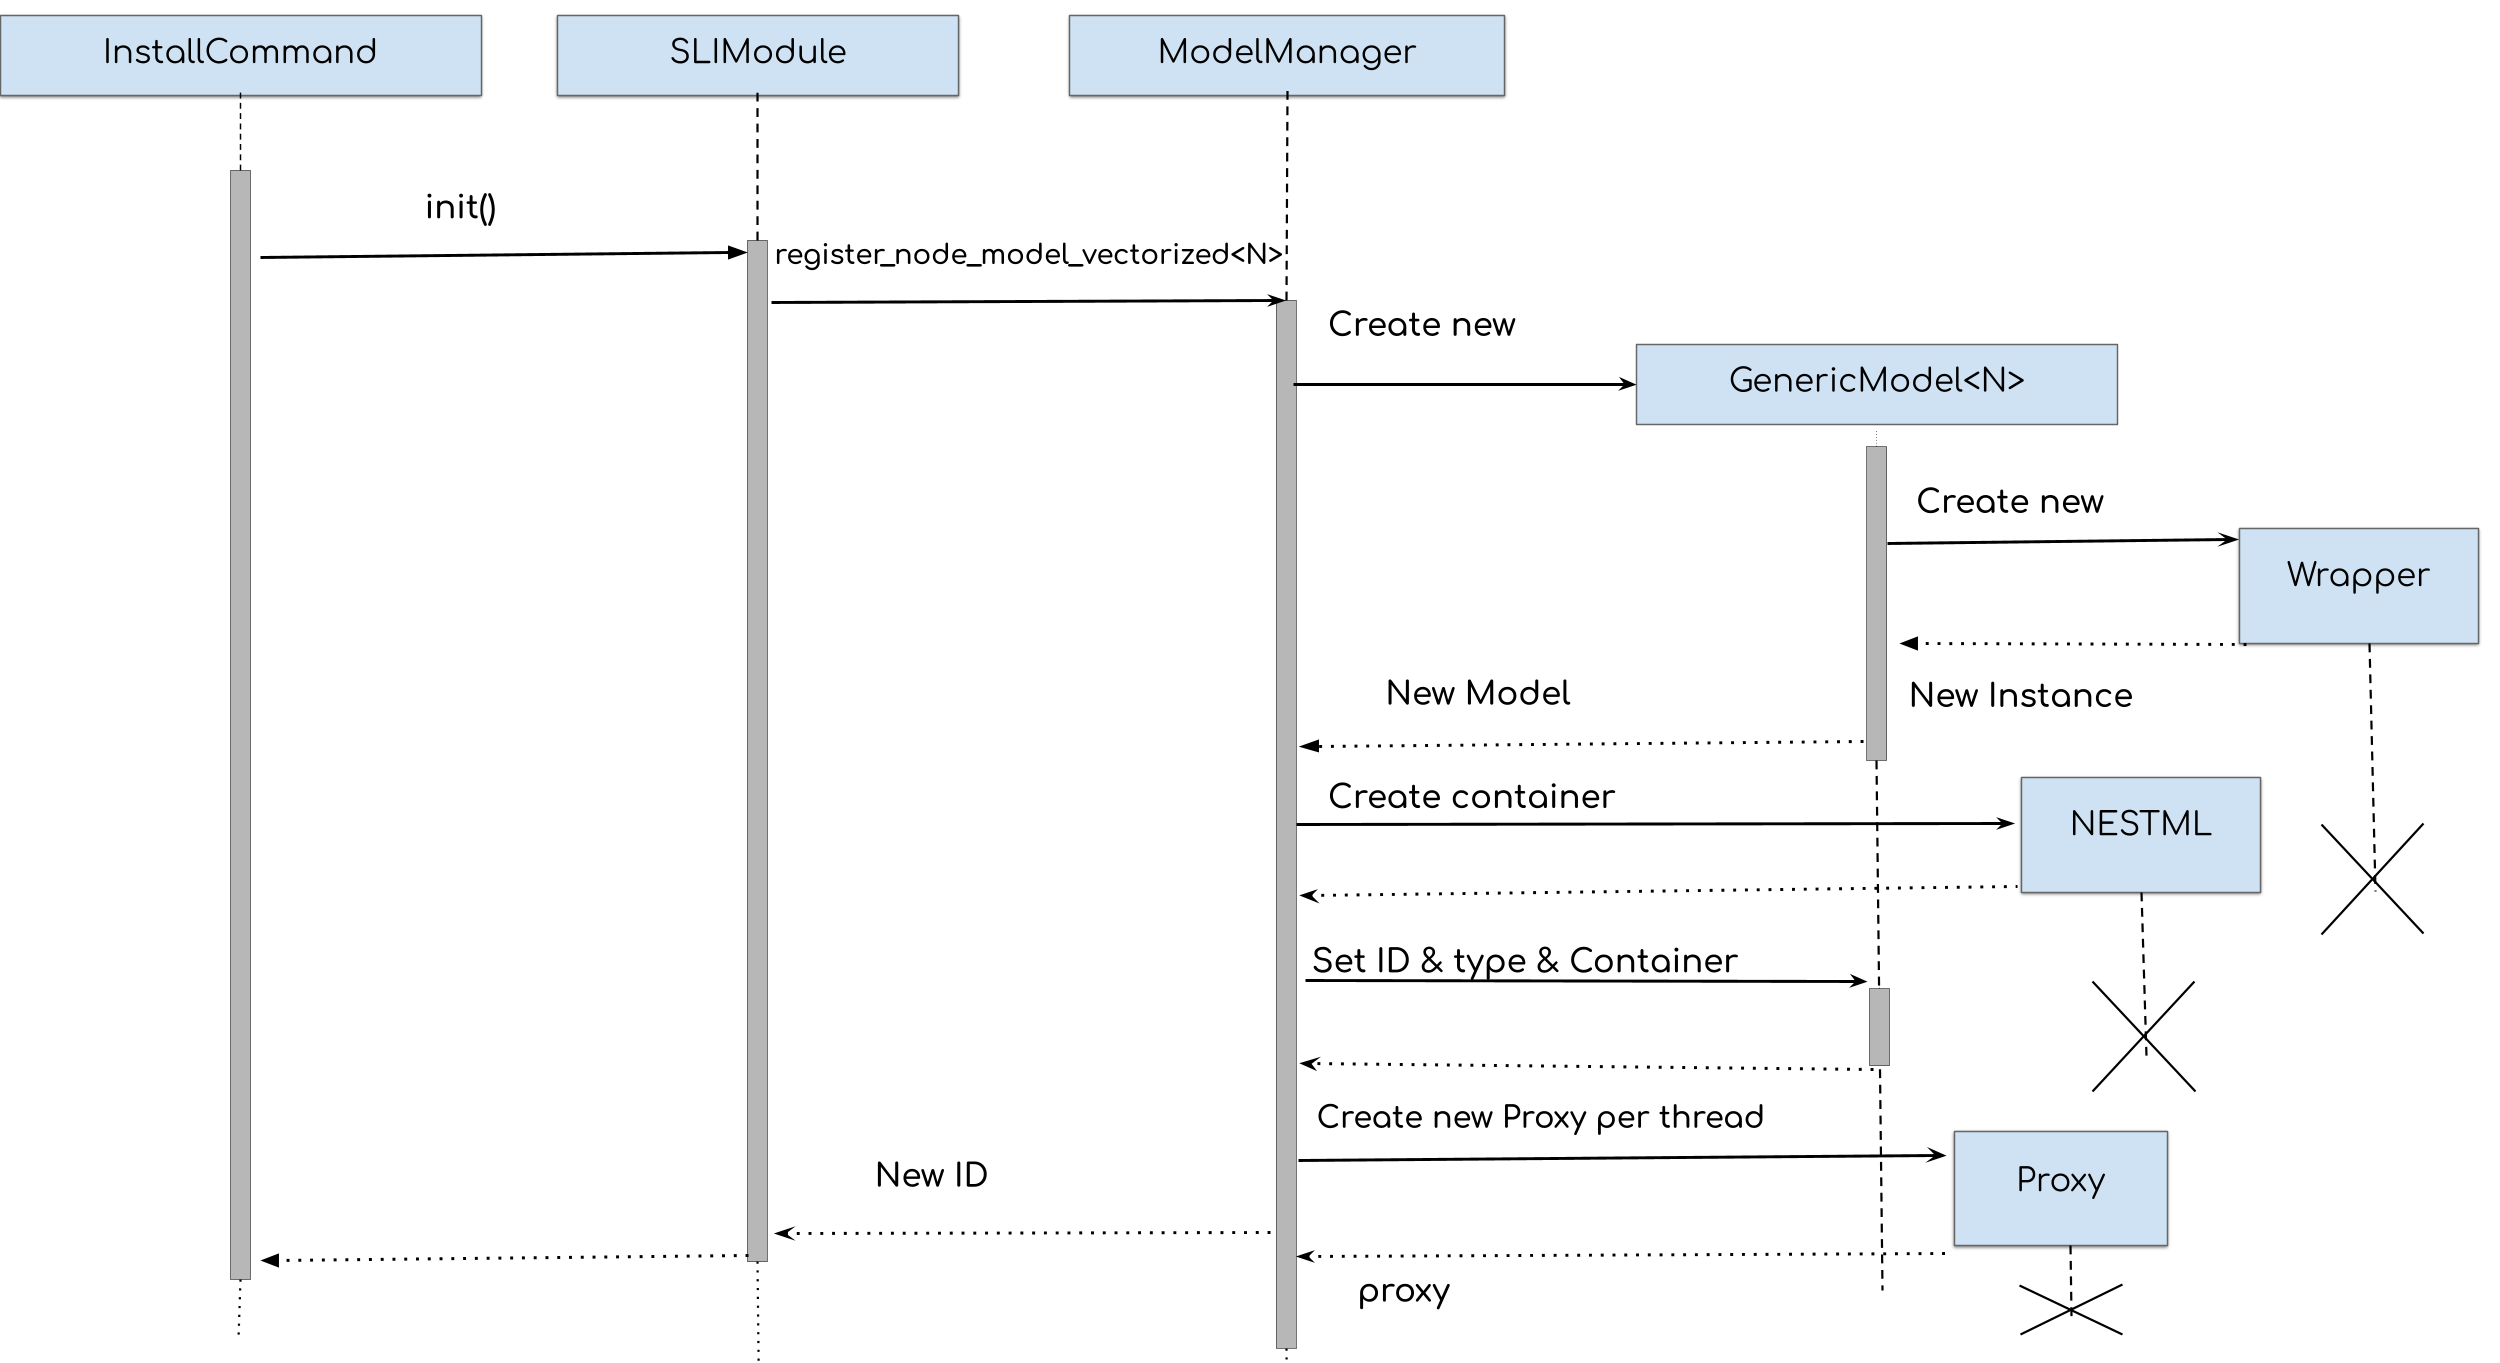
\includegraphics[width=\textwidth]{src/pic/node_creation_vec.png}
\caption{\textbf{Registering a vectorized model}: The message sequence chart depicts the interaction between the components in the NestKernel responsible for registering new custom vectorized models.}
\label{fig:register_container}
\end{figure}

As depicted in the \autoref{fig:register_container}, registering new external models in the NestKernel starts with calling the \texttt{register\_node\_model\_vectorized()} function in the \texttt{ModelManager}. The function then creates a new instance of the \texttt{GenericModel}, but instead of providing the model class type as the value of the template \texttt{T}, we set \texttt{T} to the \texttt{Wrapper}. In other words, we create an instance of type \texttt{GenericModel<Wrapper>}, which internally stores an instance of the \texttt{Wrapper}. After the constructor of the \texttt{GenericModel} finishes, the control returns to \texttt{register\_node\_model\_vectorized()}, which proceeds by creating an instance of the \texttt{VectorizedNode} which is indicated as \texttt{NESTML} in the figure. We create the container from the \texttt{VectorizedNode} and then update the created model by setting its \texttt{id}, \texttt{type} and \texttt{container}. Afterwards, as in the normal registration workflow, we create the \texttt{proxy} models for each thread. The main difference between registering a normal model and a vectorized model is thus in the class type \texttt{T} provided to the \texttt{GenericModel} and the extra step of creating the container as an instance of the \texttt{VectorizedNode} class.

In a typical simulation with external simple models without the vectorization feature, there is am important condition that must be satisfied between the created nodes and the current number of used threads. The condition states that each node exactly belongs to one thread and threads can not modify the state of nodes coming from different threads. Since the \texttt{VectorizedNode} behaves the same as the \texttt{Node} class, the same must hold for containers. Each container must belong exactly to one thread, and threads can only modify the containers they possess. In order for the \texttt{VectorizedNode} to fulfill this requirement, we have slightly modified the \texttt{Model} class and the  \texttt{add\_neurons()} function of the \texttt{ModelManager}.\\

\begin{figure}[ht!]
    \centering
    \lstset{language=C++,
                keywordstyle=\color{blue},
                stringstyle=\color{red},
                commentstyle=\color{green},
                morecomment=[l][\color{magenta}]{\#}
}
\begin{lstlisting}[caption=Assigning containers to threads,frame=tlrb, label=lst:thread_container]{Name}
if (model.get_uses_vectors())
{
    if (model.has_thread_assigned(t))
    {
        index t_container_pos = model.get_node_pos_in_thread(t);
        t_container = vectorized_nodes.at(t).at(t_container_pos);
    }
    else
    {
        t_container = model.get_container()->clone();
        t_container->set_thread(t);
        vectorized_nodes.at(t).push_back(t_container);
        index t_container_pos = vectorized_nodes.at(t).size() - 1;
        model.add_thread_node_pair(t, t_container_pos);
    }
}
\end{lstlisting}
\end{figure}

\autoref{lst:thread_container} shows the inserted functionality in the \texttt{add\_neurons()} function for creating new \texttt{Node} instances from the registered models. We start by checking if the model class supports vectorization, and if this is the case, we ask the model instance if it has seen the current running thread $t$ or not. If the model knows the thread $t$, an instance of the \texttt{VectorizedNode} was already created, and we simply ask the model to give us the position of the container in the thread $t$ and retrieve it in order to resize and adjust it accordingly. If the model has not seen the $t$ yet, we \emph{clone} the container that is stored inside the model and update it by providing the thread $t$ that is owning it and also insert the container into the thread context. To simplify the matching between containers and threads, we have an attribute called \texttt{vectorized\_nodes} in the shape of \texttt{vector < vector < VectorizedNode > >}, so that the first dimension is occupied with the thread ID and the second dimension with the created containers. The created container $c$ within the thread $t$ is then stored as \texttt{vectorized\_nodes.at(t).push(c)}, and the thread is registered in the container by simply calling \texttt{container.set\_thread(t)}. Once the matching between the container and the thread is completed, we register the thread $t$ in the model instance, so that by the next call the model knows which container to retrieve at which position.

For models that do not support vectorization, the inserted block is ignored and the function \texttt{add\_neurons()}  continues to execute without further changes. Since the \texttt{Wrapper} inherits from the \texttt{Node} class, the \texttt{create()} function inside the model always returns an instance from the provided class \texttt{T} inside the \texttt{GenericModel<T>} class, which can be either the registered model without vectorization or the new \texttt{Wrapper} class. As depicted in \autoref{lst:creating_nodes_while}, we only have minimal changes within the \texttt{while-loop}, and update the container once after the loop to avoid the overhead of repeatedly calling \texttt{resize()} on it.\\

\begin{figure}

    \lstset{language=C++,
                keywordstyle=\color{blue},
                stringstyle=\color{red},
                commentstyle=\color{green},
                morecomment=[l][\color{magenta}]{\#}
            }
\begin{lstlisting}[caption=Creating nodes,frame=tlrb, label=lst:creating_nodes_while]{Name}
while (node_id <= max_node_id)
{
    Node *node = model.create(t);

    node->set_container(t_container);
    node->set_node_id_(node_id);
    node->set_nc_(nc_ptr);
    node->set_model_id(model.get_model_id());
    node->set_thread(t);
    node->set_vp(vp);
    node->set_initialized();

    local_nodes_[t].add_local_node(*node);

    node_id += num_vps;
    has_at_leat_one_node = true;
}

local_nodes_[t].set_max_node_id(max_node_id);

if (t_container and has_at_leat_one_node)
{
    t_container->resize(max_new_per_thread, t);
}
\end{lstlisting}
\end{figure}

\section{Limitations}

So far, we only made vectorization work with \emph{multithreading}, and a full integration into the NestKernel is still pending. We have implemented the \texttt{VectorizedNode} class that represents a container holding vectors, and the size of these vectors is the number of created \texttt{Wrapper} instances pointing to the container. For simplicity, we can consider the container as an \emph{array} and the \texttt{Wrapper} instances represent each entry in the array. Thus, each \texttt{Wrapper} can only modify the entry it is pointing to. Right now, when we update the \texttt{Node} instances, we are iterating over each of them individually. For the normal models without vectorization, we can not do anything different, but for the vectorized models, we should aggregate the \texttt{Node} (i.e., \texttt{Wrapper}) instances that share the same container and then only apply the function we want on the container. Assuming we have $n$ containers and each container has $k$ \texttt{Wrapper}s pointing to it, and we have a function $f$ that is applied to these items separately, and it will be called $n\cdot k$ times in total, and for a large $k$ this might be a huge overhead. Instead, we could aggregate the items and only call the function $n$  times. Thus, each container can fully utilize the vectorization by internally applying the function $f$ in parallel to the $k$ items.

In addition, the \texttt{get\_status()} and \texttt{set\_status()} functions do not fully utilize the implemented new data structure for vectorization. Assuming the container has $n$ vectors of size $k$ ($k$ is the number of attributes in the model). The normal execution of these functions takes each \texttt{Node} instance individually and iterates over the $k$ attributes and returns a \emph{dictionary} containing the values of the $k$ attributes. This workflow does not work well with vectorization, because if each \texttt{Wrapper} within the same container executes the same logic, then we might have a high number of cache misses. Assuming we have two consecutive accesses $x_i$ and $x_{i+1}$, and we have $k$ large enough so that not all vectors can be loaded into the registers, the \texttt{Wrapper} at position $x_i$ loads its necessary data and returns the dictionary, the second \texttt{Wrapper} $x_{i+1}$ on the other hand must load the first $k$ vectors again. What really should happen is that each of the $l$ vectors must be loaded once in the registers. Since we have a consecutive access, all the entries must be loaded and ready to be used for constructing the result. Better yet, we could again group the \texttt{Wrapper} instances by the container type and let the container call these functions and treat each of these $k$ vectors individually and in parallel.

\afterpage{\blankpage}
\cleardoublepage

